\documentclass{article}
\usepackage[utf8]{inputenc}
\usepackage{tikz}
\usepackage{amssymb}
\usepackage{amsmath}
\usepackage{amssymb}

\begin{document}

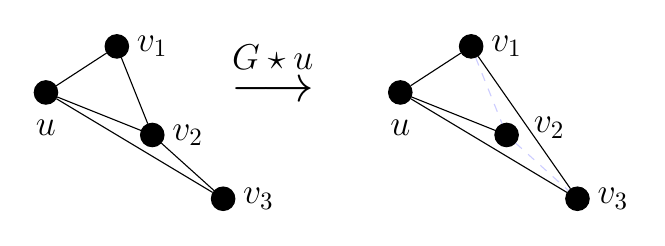
\begin{tikzpicture}[scale=0.9, transform shape]
    \node[shape=circle,draw=black,fill=black] (A) at (0,0) {};
    \node[] (u) at (0,-0.5) {\Large $u$};
    \node[shape=circle,draw=black,fill=black] (B) at (1,0.65) {};
    \node[] (v1) at (1.5,0.65) {\Large $v_1$};
    \node[shape=circle,draw=black,fill=black] (C) at (1.5,-0.6) {};
    \node[] (V2) at (2,-0.6) {\Large $v_2$};
    \node[shape=circle,draw=black,fill=black] (D) at (2.5,-1.5) {};
    \node[] (v3) at (3,-1.5) {\Large $v_3$};
    \draw[-] (A) -- (B);
    \draw[-] (A) -- (C);
    \draw[-] (A) -- (D);
    \draw[-] (B) -- (C);
    \draw[-] (C) -- (D);
    \node[] (eq) at (3.2,0) {\huge $\longrightarrow$};
    \node[] (eq) at (3.2,0.5) {\Large $G\star u$};
    
    \node[shape=circle,draw=black,fill=black] (A) at (5,0) {};
    \node[] (u) at (5,-0.5) {\Large $u$};
    \node[shape=circle,draw=black,fill=black] (B) at (6,0.65) {};
    \node[] (v1) at (6.5,0.65) {\Large $v_1$};
    \node[shape=circle,draw=black,fill=black] (C) at (6.5,-0.6) {};
    \node[] (v2) at (7.1,-0.5) {\Large $v_2$};
    \node[shape=circle,draw=black,fill=black] (D) at (7.5,-1.5) {};
    \node[] (v3) at (8,-1.5) {\Large $v_3$};
    \draw[-] (A) -- (B);
    \draw[-] (A) -- (C);
    \draw[-] (A) -- (D);
    \draw[-] (B) -- (D);
    \draw[dashed,color=white!80!blue] (B) -- (C);
    \draw[dashed,color=white!80!blue] (C) -- (D);
    
\end{tikzpicture}

\end{document}